% !TEX root = ba_doc.tex
\begin{markdown}
\section{Results} \label{results}

## Application

The user interface was designed to provide students with the familiar look and feel of a native mobile application. We chose a minimalistic design approach. The focus was on displaying relevant information without any distracting noise or clutter and a fast and intuitive user experience. Users can choose between a light theme and a dark theme (Figures \ref{fig:LoginFigure}, \ref{fig:MenuFigure} and \ref{fig:EventsFigure}). A detailed interaction flow with ZHAWo is described in the following sections.

### General

On a users first visit to ZHAWo, a prompt is shown to enter their ZHAW username (Figure \ref{fig:LoginFigure} A). A list of all available student and professor names is loaded and on user input, suggestions from that list are displayed. Since there is no persistent user specific data, setting up an account is not needed. However, the ZHAW username is required to fetch the correct timetable. This username is stored and on the next visit, the initial screen is skipped and users have immediate access to their timetable.

\begin{figure}[H]
  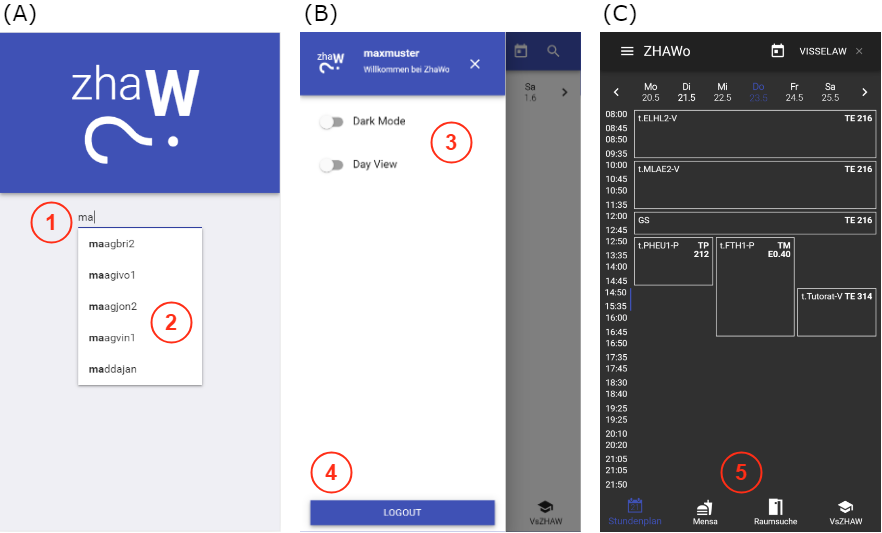
\includegraphics[width=16cm, center]{./figures/login_figure.png}
  \captionsetup{width=15.5cm}
  \caption[General user interface]{\textbf{General user interface}: \textbf{A}: On first visit, users are prompted to enter (1) and select (2) their ZHAW username. \textbf{B}: Through a collapsible application drawer, users have access to application settings (3) to change the application theme and timetable display mode. Users can clear their stored ZHAW username through a logout button (4). \textbf{C}: Users can switch between timetable, mensa menu, room search and student events contexts through labeled icons on a bottom navigation bar (5).}
  \label{fig:LoginFigure}
\end{figure}

Through a collapsible application drawer, users have access to some basic settings like switching between display modes of the timetable and changing the application theme (Figure \ref{fig:LoginFigure} B). The two timetable display modes show either the user's timetable for a single day or for a full week. The saved ZHAW username can be cleared by clicking the logout button at the bottom of the application drawer.

Switching between contexts (corresponding to the four primary functions timetable, mensa menus, room search and student events) is done through labeled icons on a navigation bar at the bottom of the screen (Figure \ref{fig:LoginFigure} C). The application state such as selected date or time frame for the room search are preserved between context switches.

### Timetable

By default, the timetable is displayed in a day view (Figure \ref{fig:TimetableFigure1} A). Individual events are displayed in their corresponding time slots. The time slots are displayed on the left with a subtle indicator for the current time slot. If there are events that run overlap in time, they are displayed next to eachother in the day view. To navigate between different dates, users can swipe their screen to the right to advance one day or swipe to the left to go to the previous day respectively. Above the timetable, a navigation bar is displayed which highlights the currently displayed day or week. As an alternative to the swipe interactions, users can directly select a date in the navigation bar or jump one week back or forward through the arrow buttons. To quickly jump to the timetable of day current day or week respectively, users can click on the calendar icon in a context action area on the top right of the screen (Figure \ref{fig:TimetableFigure1} B).

In addition to the day view, users can choose to display their timetable for a whole week. Since display space is limited especially on small mobile devices, overlapping events are shown as an indicator below the longest running event during that time frame as seen in \ref{fig:TimetableFigure1} B.

When clicking on a specific event, a modal pops up displaying detailed information about that event (Figure \ref{fig:TimetableFigure1} C).

\begin{figure}[H]
  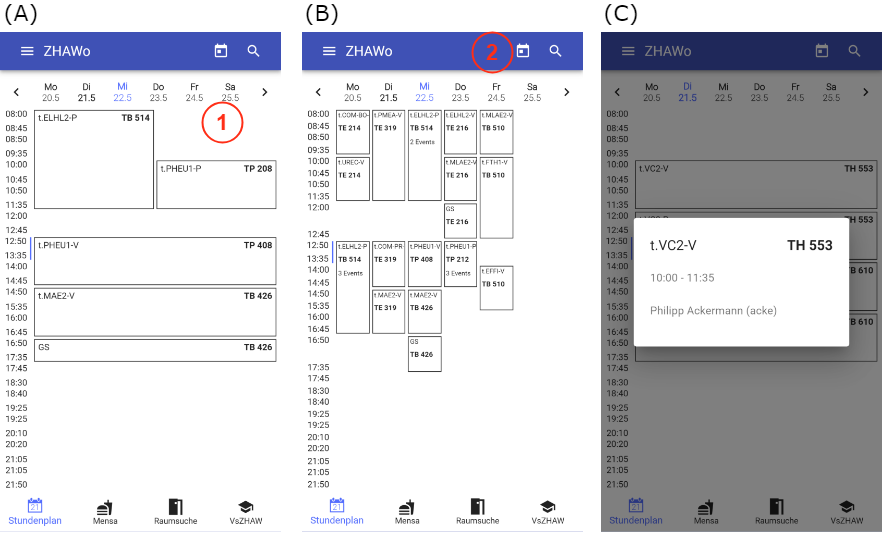
\includegraphics[width=16cm, center]{./figures/timetable_figure1.png}
  \captionsetup{width=15.5cm}
  \caption[Timetable user interface]{\textbf{Timetable user interface}: \textbf{A}: Day view of a users timetable with overlapping events from 10:00 to 11:35. Navigation bar to navigate to specific dates and to navigate between weeks (1). Alternatively, navigation between days or weeks can be achieved through swipe gestures. \textbf{B}: Week view of a users timetable with overlapping event indicators and context action area button to jump to current date (2). \textbf{C}: Detail modal of a specific event. Is opened when user clicks on event from either day or week view.}
  \label{fig:TimetableFigure1}
\end{figure}

Users can also search for and display other timetables than their own. Through a search icon button in the context action area, a modal can be opened where users can search for and display timetables of other students, lecturers, classes, courses or rooms (Figure \ref{fig:TimetableFigure2} A and B). The currently displayed search timetable can be cleared through the indicator in the context action area (Figure \ref{fig:TimetableFigure2} C).

\begin{figure}[H]
  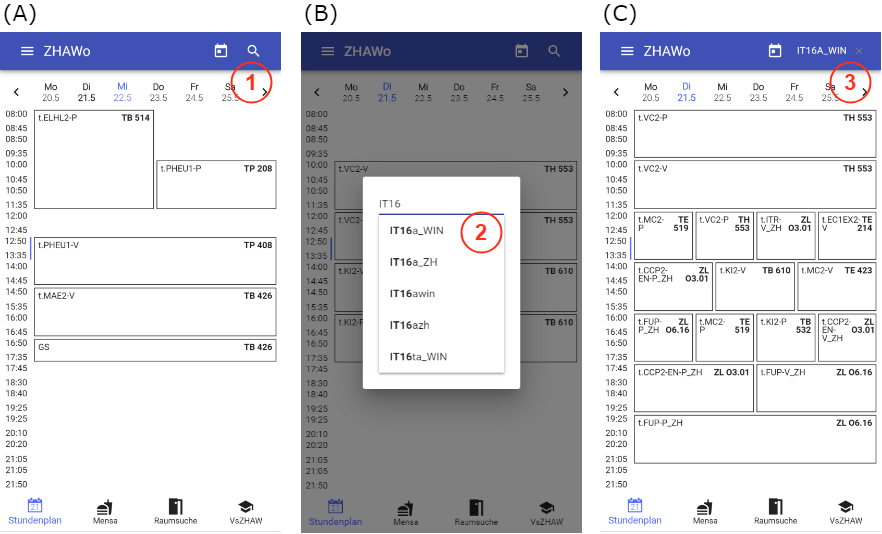
\includegraphics[width=16cm, center]{./figures/timetable_figure2.png}
  \captionsetup{width=15.5cm}
  \caption[Timetable search user interface]{\textbf{Timetable search user interface}: \textbf{A}: Default user timetable with search icon button in context action area to open search modal (1). \textbf{B}: Search modal with suggestions for students, lecturers, classes, courses and rooms (2). \textbf{C}: Search timetable for specific class with indicator and clear button (3) in context action area.}
  \label{fig:TimetableFigure2}
\end{figure}

### Mensa menus

The mensa menus are displayed as a list of available menus with their category, menu name and description and ZHAW internal prices. The title indicates the mensa where the currently displayed menu is available. Through a mensa icon in the context action area, users can select all mensas with menu information available (Figure \ref{fig:MenuFigure} A and B). Navigation between menus of different days is consistent with the navigation for the timetable context, with a navigation bar in addition to swipe gestures.

\begin{figure}[H]
  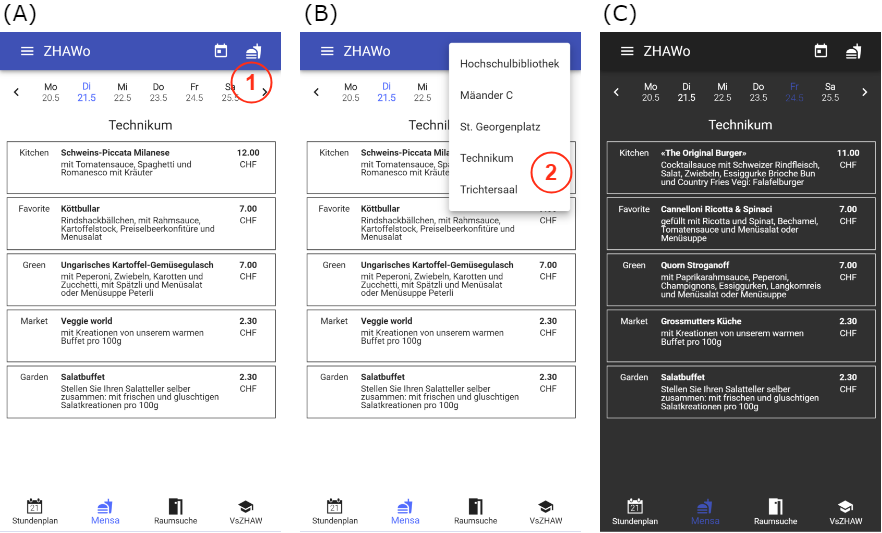
\includegraphics[width=16cm, center]{./figures/menu_figure.png}
  \captionsetup{width=15.5cm}
  \caption[Mensa menu user interface]{\textbf{Mensa menu user interface}: \textbf{A}: Mensa menu for the Technikum mensa with menu category, name, description and ZHAW internal prices. Title indicates currently displayed mensa which can be changed through the mensa icon in the context action area (1). \textbf{B}: Mensa selection (2). \textbf{C}: Dark theme mensa menu display.}
  \label{fig:MenuFigure}
\end{figure}

### Room search

To search for currently unoccupied rooms at the ZHAW School of Engineering, users can enter a time range during which they want to use the room (Figure \ref{fig:RoomSearchFigure} A). Once they've entered the start and end time, the can press the search button and the free rooms will be filtered to only show rooms that are unoccupied during the correct time slots. To browse the free rooms, users can navigate through a map of the School Of Engineering campus showing all buildings. Buildings highlighted in blue have at least one free room during the entered time range (Figure \ref{fig:RoomSearchFigure} B). To see which rooms are free, users can click on a building on the map, and a floor plan of that building will appear with labeled and highlighted free rooms. They can navigate through the different floors with the buttons above the floor plans. The individual floor plans show which rooms are free and where they are (Figure \ref{fig:RoomSearchFigure} C). To switch to a different building, users can navigate back to the campus overview map through the School Of Engineering button next to the floor navigation.

\begin{figure}[H]
  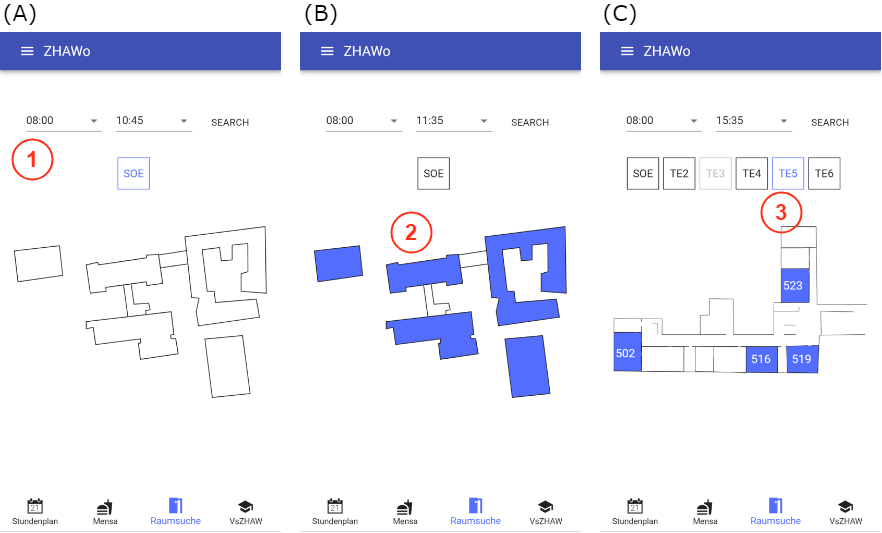
\includegraphics[width=16cm, center]{./figures/roomsearch_figure1.png}
  \captionsetup{width=15.5cm}
  \caption[Room search user interface]{\textbf{Room search user interface}: \textbf{A}: Initial screen of the room search without an active search with input for start and end time and search button (1). \textbf{B}: Campus overview map of the School Of Engineering with buildings highlighted in blue that contain a free room in the entered time range. By clicking on a building on the map, users get directed to the respective floor plans of that building (2). \textbf{C}: Detailed floor plan of TE building with free rooms highlighted and labeled. Navigation through different floors with buttons above the map (3).}
  \label{fig:RoomSearchFigure}
\end{figure}

### Student events

Users can browse vszhaw news and events through a chronological list of blog posts. Full news posts are linked and can be reached by clicking an the individual posts. If there is an upcoming event in the official vszhaw calendar, it will be featured above the news feed (Figure \ref{fig:EventsFigure} A and B). Additionaly, student events are displayed as a banner in the timetable context of their date (Figure \ref{fig:EventsFigure} C). Both banner and student event feature are linked to more detailed information about the event on the vszhaw website.

\begin{figure}[H]
  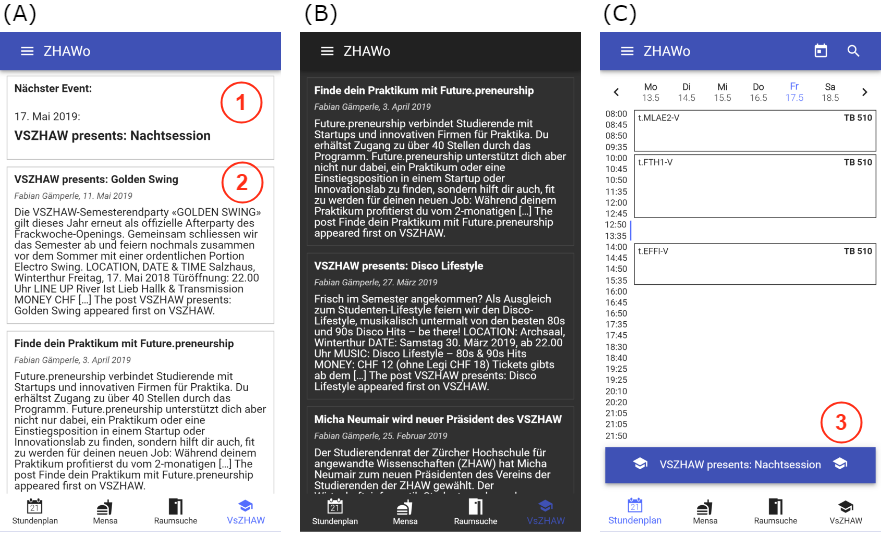
\includegraphics[width=16cm, center]{./figures/events_figure.png}
  \captionsetup{width=15.5cm}
  \caption[Student events user interface]{\textbf{Student events user interface}: \textbf{A}: Vszhaw student events (1) and news feed (2). \textbf{B}: Dark theme version of vszhaw news feed. \textbf{C}: Student event banner in the timetable context (3).}
  \label{fig:EventsFigure}
\end{figure}

\newpage

\end{markdown}

